%&<latex>
\documentclass[letterpaper,12pt]{article}

%%%%%%%%%%%%%%%%%%%%%%%%%%%%%%%%%%%%%%%%%%%%%%%%%%%%%%%%%%%%
%% preamble %%%%%%%%%%%%%%%%%%%%%%%%%%%%%%%%%%%%%%%%%%%%%%%%
\pdfpagewidth = 8.5in
\pdfpageheight = 11.0in
\usepackage[left=1in,right=1in,top=1in,bottom=1in]{geometry}

\pagestyle{plain}
\pagenumbering{arabic}
\usepackage{setspace}
\usepackage[fleqn]{amsmath}
\usepackage{amssymb}
\usepackage{graphicx}
\usepackage{url}
\usepackage{verbatim}
\usepackage[title]{appendix}
\usepackage{indentfirst}
\usepackage{booktabs}
\usepackage{multirow}
\usepackage{ragged2e}
\setlength{\RaggedRightParindent}{\parindent}
\usepackage{upgreek}
\usepackage[T1]{fontenc}
\usepackage[titles]{tocloft}
\usepackage{xspace}
\usepackage[usenames]{color}
\usepackage{ifthen}
\usepackage{cancel}
\usepackage{array}
\usepackage{tabulary}
\usepackage{authblk}
\usepackage{tikz}
\usepackage[normalem]{ulem}

%% Set up color palettes %%%%%%%%%%%%%%%%%%%%%%%%%%%%%%%%%%%%%%%%%%%%
% Color palette GreenOrange_6 from
% https://jiffyclub.github.io/palettable/tableau/
\definecolor{pgreen}     {RGB}{50,162,81}
\definecolor{porange}    {RGB}{255,127,15}
\definecolor{pblue}      {RGB}{60,183,204}
\definecolor{pyellow}    {RGB}{255,217,74}
\definecolor{pteal}      {RGB}{57,115,124}
\definecolor{pauburn}    {RGB}{184,90,13}
%%%%%%%%%%%%%%%%%%%%%%%%%%%%%%%%%%%%%%%%%%%%%%%%%%%%%%%%%%%%%%%%%%%%%

\usepackage{hyperref}
\hypersetup{pdfborder={0 0 0},
            % colorlinks=true,
            colorlinks=false,
            urlcolor=porange,
            linkcolor=pauburn,
            citecolor=pteal}

\usepackage[capitalize]{cleveref}
\newcommand{\crefrangeconjunction}{--}

% Set up line numbering; using lineno to number lines of paragraphs with
% equations sanely
\usepackage[right, mathlines]{lineno}
\setlength\linenumbersep{1cm}
\def\linenumberfont{\normalfont\scriptsize\sffamily}

% Set up caption formatting
\usepackage{subcaption}
\usepackage[format=plain, labelsep=period, singlelinecheck=true, skip=2pt, font=sf]{caption}
\DeclareCaptionLabelFormat{noSpace}{{#1}{#2}}
\DeclareCaptionListFormat{figList}{Figure {#2}.}
\DeclareCaptionListFormat{sFigList}{Figure S{#2}.}
\DeclareCaptionListFormat{aFigList}{Figure A{#2}.}

% Define tightly formated list environments via enumitem
\usepackage{enumitem}
\newenvironment{tightItemize}{%
\begin{itemize}[noitemsep, topsep=0pt, parsep=0pt, partopsep=0pt]}
{\end{itemize}}

\newenvironment{veryTightItemize}{%
\begin{itemize}[noitemsep, topsep=0pt, parsep=0pt, partopsep=0pt, leftmargin=*]}
{\end{itemize}}

\newenvironment{tightEnumerate}{%
\begin{enumerate}[noitemsep, topsep=0pt, parsep=0pt, partopsep=0pt]}
{\end{enumerate}}

\newenvironment{veryTightEnumerate}{%
\begin{enumerate}[noitemsep, topsep=0pt, parsep=0pt, partopsep=0pt, leftmargin=*]}
{\end{enumerate}}

\newcommand{\citationNeeded}{\textcolor{magenta}{\textbf{[CITATION NEEDED!]}}\xspace}
\newcommand{\tableNeeded}{\textcolor{magenta}{\textbf{[TABLE NEEDED!]}}\xspace}
\newcommand{\figureNeeded}{\textcolor{magenta}{\textbf{[FIGURE NEEDED!]}}\xspace}
\newcommand{\highLight}[1]{\textcolor{magenta}{\MakeUppercase{#1}}}

\newcommand{\editorialNote}[1]{\textcolor{red}{[\textit{#1}]}}
\newcommand{\ignore}[1]{}
\newcommand{\addTail}[1]{\textit{#1}.---}
\newcommand{\super}[1]{\ensuremath{^{\textrm{#1}}}}
\newcommand{\sub}[1]{\ensuremath{_{\textrm{#1}}}}
\newcommand{\dC}{\ensuremath{^\circ{\textrm{C}}}}
\newcommand{\tb}{\hspace{2em}}
\newcommand{\tn}{\tabularnewline}
\newcommand{\spp}[1]{\textit{#1}}

\providecommand{\e}[1]{\ensuremath{\times 10^{#1}}}

\newcommand{\change}[2]{{\color{red} #2}\xspace}
\newcommand{\thought}[1]{\textcolor{purple}{THOUGHT: #1}}

\newcommand{\widthFigure}[5]{\begin{figure}[htbp]
\begin{center}
    \includegraphics[width=#1\textwidth]{#2}
    \captionsetup{#3}
    \caption{#4}
    \label{#5}
    \end{center}
    \end{figure}}

\newcommand{\heightFigure}[5]{\begin{figure}[htbp]
\begin{center}
    \includegraphics[height=#1]{#2}
    \captionsetup{#3}
    \caption{#4}
    \label{#5}
    \end{center}
    \end{figure}}

\newcommand{\smartFigure}[4]{%
    \begin{figure}[htbp]
        \begin{center}
            \includegraphics[width=\textwidth,height=0.95\textheight,keepaspectratio]{#1}
            \captionsetup{#2}
            \caption{#3}
            \label{#4}
        \end{center}
    \end{figure}
}

\newcommand{\mFigure}[3]{\smartFigure{#1}{listformat=figList}{#2}{#3}\clearpage}
\newcommand{\embedFigure}[3]{\smartFigure{#1}{listformat=figList}{#2}{#3}}
\newcommand{\siFigure}[3]{\smartFigure{#1}{name=Figure S, labelformat=noSpace, listformat=sFigList}{#2}{#3}\clearpage}
\newcommand{\appendixFigure}[3]{\smartFigure{#1}{name=Figure A, labelformat=noSpace, listformat=aFigList}{#2}{#3}\clearpage}
\newcommand{\embedAppendixFigure}[3]{\smartFigure{#1}{name=Figure A, labelformat=noSpace, listformat=aFigList}{#2}{#3}}

\newcommand{\given}{\ensuremath{\,|\,}\xspace}

\newcommand{\topology}{\ensuremath{T}\xspace}
\newcommand{\data}{\ensuremath{D}\xspace}
\newcommand{\flipdata}{\ensuremath{D}\xspace}
\newcommand{\model}[1][]{\ensuremath{M_{#1}}\xspace}
\newcommand{\coinmodel}[1][]{\ensuremath{M_{#1}}\xspace}
\newcommand{\parameters}[1][]{\ensuremath{\theta_{#1}}\xspace}
\newcommand{\dparameters}[1][]{\ensuremath{\psi_{#1}}\xspace}
\newcommand{\evoparameters}[1][]{\ensuremath{\theta_{#1}}\xspace}
\newcommand{\branchlengths}[1][]{\ensuremath{\lambda_{#1}}\xspace}
\newcommand{\probheads}[1][]{\ensuremath{\theta_{#1}}\xspace}
\newcommand{\diff}[1]{\ensuremath{\mathrm{d}#1}}
\newcommand{\nmodels}{\ensuremath{N}\xspace}
\newcommand{\pvar}[1][]{\ensuremath{Pvar_{#1}}\xspace}


\usepackage[round]{natbib}

\newcommand{\vmdel}[1]{\sout{#1}}
\newcommand{\vmadd}[1]{\textbf{\color{red}{#1}}}
\newcommand{\vmcomment}[1]{({\color{magenta}{VM's comment:}} \textbf{\color{magenta}{#1}})}
\newcommand{\jrocomment}[1]{({\color{green}{JRO's comment:}} \textbf{\color{green}{#1}})}



% \title{Integrals, lots of integrals}
\title{Marginal likelihoods in phylogenetics: a review of methods and applications}

\author[1]{Jamie R.\ Oaks\thanks{Corresponding author: \href{mailto:joaks@auburn.edu}{\tt joaks@auburn.edu}}}
\author[2]{Kerry A.\ Cobb}
\author[3]{Vladimir N.\ Minin}
\author[4]{Adam D.\ Leach\'{e}}
\affil[1,2]{Department of Biological Sciences \& Museum of Natural History, Auburn University, Auburn, Alabama 36849}
\affil[3]{Department of Statistics, University of California, Irvine, California 92697}
\affil[4]{Department of Biology \& Burke Museum of Natural History and Culture, University of Washington, Seattle, Washington 98195}

% \date{\today}
\date{\parbox{\linewidth}{\centering%
    \today\endgraf\bigskip
    \textbf{Running head}: Marginal likelihoods in phylogenetics}}

\makeatletter
\let\msTitle\@title
\let\msAuthor\@author
\let\msDate\@date
\makeatother
%%%%%%%%%%%%%%%%%%%%%%%%%%%%%%%%%%%%%%%%%%%%%%%%%%%%%%%%%%%%
%%%%%%%%%%%%%%%%%%%%%%%%%%%%%%%%%%%%%%%%%%%%%%%%%%%%%%%%%%%%

\begin{document}
% \doublespacing
% \begin{linenumbers}

\maketitle

\begin{abstract}
    By providing a framework of accounting for the shared ancestry inherent to all
life,
phylogenetics is becoming the statistical foundation of biology.
The importance of model choice continues to grow as phylogenetic models
continue to increase in complexity to better capture micro and
macroevolutionary processes.
% A Bayesian approach to such rich models is often necessary to make them
% tractible.
In a Bayesian framework, 
the marginal likelihood is how data update our prior beliefs about models,
which gives us an intuitive measure of comparing model fit that is grounded in
probability theory.
Given the rapid increase in the number and complexity of phylogenetic models,
methods for approximating marginal likelihoods is increasingly important.
Here we try to provide an intuitive description of marginal likelihoods and why
they are important in Bayesian model testing.
We also categorize and review methods for estimating marginal likelihoods of
phylogenetic models.
In doing so, we use simulations to evaluate the performance of one such method
based on approximate-Bayesian computation (ABC) and find that is biased as
predicted from theory.
Furthermore, we review some applications of marginal likelihoods to
phylogenetics, highlighting how they can be used to learn about models of
evolution from biological data.
We conclude by discussing the challenges of Bayesian model choice and future
directions that promise to improve the approximation of marginal likelihoods
and Bayesian phylogenetics as a whole.


    \vspace{12pt}
    \noindent\textbf{KEY WORDS: phylogenetics, marginal likelihood, model choice} 
\end{abstract}

\newpage

\section{Introduction}

Phylogenetics is rapidly progressing as the statistical foundation of
comparative biology, providing a framework for accounting for the shared
ancestry inherent in biological data.
Soon after phylogenetics became feasible as a likelihood-based statistical
endeavor \citep{Felsenstein1981}, models started becoming richer to better
capture processes of biological diversification and character change.
This trend in model complexity made Bayesian approaches appealing, because they
can render inference under rich models practical by leveraging prior
information and numerical techniques (e.g., data augmentation).

From the earliest days of Bayesian phylogenetics \citep{Rannala1996,Mau1997},
the numerical tool of choice for approximating the posterior distribution was
Markov chain Monte Carlo (MCMC).
By only considering the ratios of posterior densities, MCMC can avoid
calculating the proportionality constant in the denominator of Bayes' rule.
This proportionality constant is better known as the marginal likelihood---the
probability of the data under the model, averaged, with respect to the prior,
over the whole parameter space.
This marginalized measure of model fit cannot be solved analytically due to
the large number of parameters in phylogenetic models that need to be summed or
integrated.

Marginal likelihoods are central to model comparison in a Bayesian framework.
Thus, we cannot avoid calculating them if we want to be able to compare the fit
of phylogenetic models.
As the diversity and richness of phylogenetic models has increased, there has
been a renewed appreciation of the importance of such Bayesian model
comparison.
As a result, there has been a lot of work over the last decade to develop
methods for estimating marginal likelihoods of phylogenetic models.

Perhaps the simplest numerical approximation of the marginal likelihood is to
draw samples of a model's parameters from their respective prior distributions.
This turns the intractable integral into a sum of the samples' likelihoods.
Because the prior weight of each sample is one in this case, the marginal
likelihood can be approximated by simply calculating the average likelihood of
the prior samples.
Similarly, if we have a sample of the parameters from the posterior
distribution---like one would obtain from a ``standard'' Bayesian phylogenetic
analysis via MCMC---we can again use summation to approximate the integral.
The weight of each sample is the ratio of the prior density to the posterior
density.
As a result, the sum simplifies to the harmonic mean (HM) of the likelihoods
from the posterior sample \citep{Newton1994}.
Both of these techniques are importance-sampling approximations, and suffer
from the fact that the prior and posterior are often \emph{very} divergent,
with the latter usually \emph{much} more peaked than the former.
A finite sample from the prior will often yield an underestimate of the
marginal likelihood, because the region of parameter space with high likelihood
is likely to be missed.
Whereas a finite sample from the posterior will almost always lead to an
overestimate, because it will contain very few samples outside of the region of
high likelihood, where the prior has a strong downward ``pull'' on the average
likelihood.

Recent methods developed to estimate marginal likelihoods generally fall into
two categories of how to deal with the sharp contrast between the prior
and posterior that cripples the simple importance-sampling approaches
mentioned above.
One general strategy is to turn the giant leap between the unnormalized
posterior and prior into many small steps along a series of power posterior
distributions.
The second strategy is to turn the giant leap between the posterior and prior
into a smaller leap between the posterior and a reference distribution that is
as similar as possible to the posterior.
These approaches are not mutually exclusive (e.g., see Fan et al.\
\citeyear{Fan2011}), but they serve as a useful way to categorize marginal
likelihood approximation methods.
In practical terms, the first strategy is computationally expensive, because
samples need to be collected from each of the power posterior distributions,
which is not part of a ``standard'' Bayesian phylogenetic analysis.
The second strategy is very inexpensive because it attempts to approximate the
marginal likelihood using only the posterior samples collected from a
``standard'' analysis.

The goals of this review are to \ldots

\subsection{Approaches that use only posterior samples}

\begin{itemize}
    \item Generalized harmonic mean (GHM) \citep{Gelfand1994}
    \item Inflated density ratio \citep{Arima2012}
\end{itemize}

\subsection{Approaches that use power posterior samples}

\begin{itemize}
    \item Path-sampling \citep{Lartillot2006}
    \item Stepping-stone \citep{Xie2011}
    \item Generalized stepping stone \citep{Fan2011}
\end{itemize}

\subsection{Other approaches that don't fit my dichotomy}

\begin{itemize}
    \item Sequential stochastic approximation Monte Carlo (SSAMC)
        \citep{Liang2007,Cheon2008}
    \item Sequential Monte Carlo (SMC) \citep{Jordan2012}
    \item Direct sampling (model averaging)
    \item Approximate-likelihood Bayesian approaches. Wegmann's ABCToolbox
        approximates the posterior distribution with a GLM, and then takes the
        marginal of that distribution. Knowles' lab is using this to compare
        different phylogeographic models. It would be interesting to know how
        accurate these marginal likelihoods are (my guess is that they are are
        not so good). As far as I'm aware there have been no analyses to assess
        this.
\end{itemize}


\section{Acknowledgments}
We thank Mark Holder for helpful discussions about comparing approximate and
full marginal likelihoods.
We also thank Ziheng Yang and members of the Phyletica Lab (the phyleticians)
for helpful comments that improved an early draft of this paper.
The computational work was made possible by the Auburn University (AU) Hopper
Cluster supported by the AU Office of Information Technology.
% This work was possible thanks to funding provided to JRO from the National
% Science Foundation (DBI 1308885 and DEB 1656004).
This paper is contribution number \highLight{XXXX} of the Auburn University
Museum of Natural History.


\bibliographystyle{bib/sysbio}
\bibliography{bib/references}

%% LIST OF FIGURES %%%%%%%%%%%%%%%%%%%%%%%%%%
\newpage
\singlespacing

\renewcommand\listfigurename{Figure Captions}
\cftsetindents{fig}{0cm}{2.2cm}
\renewcommand\cftdotsep{\cftnodots}
\setlength\cftbeforefigskip{10pt}
\cftpagenumbersoff{fig}
\listoffigures


% \end{linenumbers}

%% TABLES %%%%%%%%%%%%%%%%%%%%%%%%%%%%%%%%
\newpage
\singlespacing

\input{tables.tex}

\clearpage

%% FIGURES %%%%%%%%%%%%%%%%%%%%%%%%%%%%%%%%
\newpage

\mFigure{images/abc-glm-bayes-factors.pdf}{
    A comparison of the approximate-likelihood Baysian computation general
    linear model (ABC-GLM) estimator of the marginal likelihood
    \citep{Leuenberger2010} to quadrature integration approximations
    \citep{Xie2011} for 100 simulated datasets.
    We compared the ratio of the marginal likelihood (Bayes factor) comparing
    the correct branch-length model
    [branch length $\sim$ uniform(0.0001, 0.1)]
    to a model with a boader prior on the branch length
    [branch length $\sim$ uniform(0.0001, 0.2)].
    The solid line represents perfect performance of the ABC-GLM estimator
    (i.e., matching the ``true'' value of the Bayes factor).
    The dashed line represents the expected Bayes factor when failing to
    penalize for the extra parameter space (branch length 0.1 to 0.2) with
    essentially zero likelihood.
    Quadrature integration with 1,000 and 10,000 steps using the rectangular
    and trapezoidal rule produced identical values of log marginal likelihoods
    to at least five decimal places for all 100 simulated datasets.
}{fig:glmPerformance}


%%%%%%%%%%%%%%%%%%%%%%%%%%%%%%%%%%%%%%%%%%%%%%%%%%%%%%%%%%%%%%%%%%
%% SUPPORTING INFO %%%%%%%%%%%%%%%%%%%%%%%%%%%%%%%%%%%%%%%%%%%%%%%
\setcounter{figure}{0}
\setcounter{table}{0}
\setcounter{page}{1}
\setcounter{section}{0}

\singlespacing

\section*{Supporting Information}
% PUT MAIN TEXT CITATION HERE
\hangindent=1cm
\noindent Title: \msTitle

\bigskip
{\noindent Authors: \msAuthor}

\newpage
\singlespacing

We set up a simple scenario for assessing the performance of the method for
estimating marginal likelihoods based on approximating the likelihood function
with a general linear model (GLM) fitted to posterior samples collected via
approximate-likelihoood Bayesian computation (ABC) \citep{Leuenberger2010};
hereforth referred to as ABC-GLM.
The scenario is a DNA sequence, 10,000-nucleotides in length, that evolves
along a branch according to a Jukes-Cantor continuous-time Markov chain (CTMC)
model of nucleotide substitution \citep{JC1969}.
Because the Jukes-Cantor model forces the relative rates of change among the
four nucleotides and the equilibrium nucleotide frequencies to be equal, there
is only a single parameter in the model, the length of the branch, and the
direction of evolution along the branch does not matter.

\subsection{Simulating data sets}
We simulated 100 data sets under this model by
\begin{enumerate}
    \item drawing 10,000 nucleotides of the ``ancestral'' sequence from their
        equilibrium frequencies ($\frac{1}{4}$), 
    \item drawing a branch length $\sim$ uniform(0.0001, 0.1), and
    \item evolving the sequence along the branch according to the Jukes-Cantor
        CTMC model to get the ``descendant'' sequence.
\end{enumerate}
This was done using the DendroPy phylogenetic API (version 4.3.0 commit
72ce015) \citep{Sukumaran2010}.

\subsection{Calculating ``true'' Bayes factors}
For each data set, we used quadrature approaches to approximate the marginal
likelihood by integrating the posterior density over the branch length prior.
We did this for two models:
\begin{enumerate}
    \item the correct model [branch length $\sim$ uniform(0.0001, 0.1)], and
    \item a model with a branch length prior slightly more than twice as broad
        [branch length $\sim$ uniform(0.0001, 0.2)], which we refer to as the
        ``vague model''.
\end{enumerate}
For both models and for each dataset we used the rectangular and trapezoidal
quadrature rules with 1,000 and 10,000 steps (i.e., four approximations of the
marginal likelihood for each data set under each model).
Across all 100 data sets and both models, all four approximations were
identical to at least five decimal places.
For each data set, we calculated the log Bayes factor comparing the correct
model to the vague model.

\subsection{Approximate-likelihood Bayesian computation}
To collect an approximate posterior sample from the correct model for a data
set, we first calculated the proportion of variable sites (\pvar) between the
two sequences.
Next, we simulated 50,000 datasets under the correct model, calculated \pvar
for each of them, and retained the 1,000 samples with the values of \pvar
closest to that calculated from the data.
Lastly, we used ABCtoolbox version 1.1 \cite{ABCtoolbox} to fit a GLM to the
retained samples and calculate the marginal density of the GLM, using a
bandwidth of 0.002.
We did the same to obtain an ABC-GLM estimate of the marginal density
for the vague model with two differences:
(1) we drew the branch length for each prior sample from the vague prior
[branch length $\sim$ uniform(0.0001, 0.2)], and
(2) to maintain the same expected tolerance under both models, we simulated
100,000 datasets under the vague model (retaining the 1,000 samples closest to
the \pvar of the data).

For each data set, we calculated the log Bayes factor from the GLM marginal
densities of the correct and vague model, and compared the ABC-GLM-estimated
Bayes factor to the ``true'' Bayes factor calculated via quadrature
integration (Figure~\ref{fig:glmPerformance}).

\subsection{Full-likelihood Markov chain Monte Carlo analyses}
One goal of the simplicity of the above model is that the additional
approximation of the ABC approach would be limited.
All numerical Bayesian analyses, based on full or approximate likelihoods,
suffer from Monte Carlo error associated with approximating the posterior with
a finite number of samples.
Approximate-likelihood methods usually suffer from two additional sources of
approximation:
(1) the full data are replaced with insufficient summary statistics, and
(2) samples are retained that do not exactly match the data or summary
statistics (i.e., the ``tolerance'' of ABC).
In our analyses described above, we avoided the former source of error by
using a sufficient statistic.
We hoped to minimize the latter source of error by evaluating many samples from
a one-dimensional model with finite bounds; we also kept this source of error
approximately equal for both models by sampling in proportion to the width of
the model.

To verify that the error introduced by the tolerance of the ABC analyses was
minimal, we compared the branch length estimates to those estimated by
full-likelihood Markov chain Monte Carlo (MCMC).
For each data set, under both models, we ran a chain for 10,000 generations,
sampling every 10 generations.
All chains appeared to reach stationarity by the first sample (10th
generation).
We plotted the branch length estimated via ABC-GLM and MCMC under both
the true and vague models against the true branch lengths.
The results of all four analyses across all 100 data sets are almost
indistinguishable (Figure~A\ref{fig:branchLengthEstimates}), confirming that
the approximation introduced by the tolerance is very minimal.
Our ABC-GLM analyses are essentially equivalent to full-likelihood Bayesian
analyses, creating a ``best-case scenario'' for evaluating the marginal
likelihood estimates of the ABC-GLM method.

\embedAppendixFigure{images/branch-length-estimates.pdf}{
    A comparison of the true branch length separating each pair of simulated
    sequences to the branch length estimated by ABC-GLM and full-likelihood
    MCMC under the correct branch-length model (branch length $\sim$ uniform(0.0001,
    0.1)) and the vague model (branch length $\sim$ uniform(0.0001, 0.1)).
}{fig:branchLengthEstimates}

\subsection{Reproducibility}
All of the code to replicate our results is freely available at
\href{https://github.com/phyletica/abc-glm-marginal-test}{https://github.com/phyletica/abc-glm-marginal-test}.

\clearpage

\input{si-tables.tex}
\clearpage

\begin{figure}[htbp]
    \begin{subfigure}[b]{0.5\textwidth}
        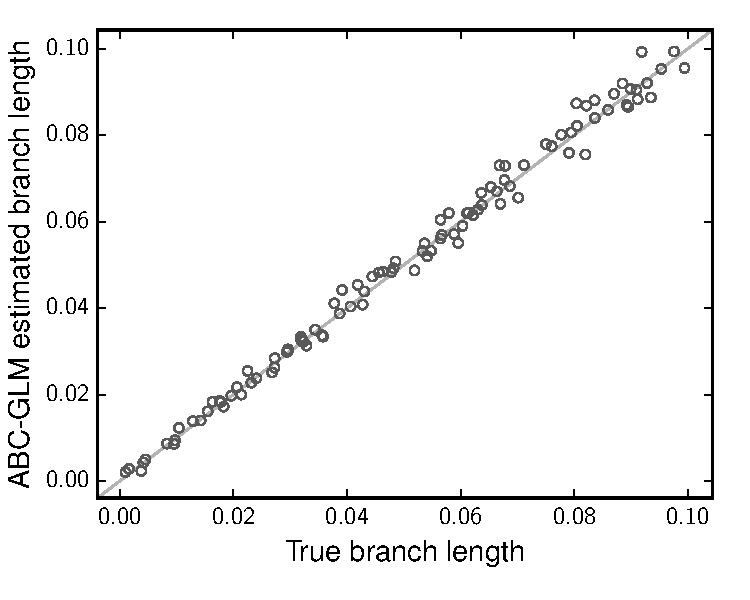
\includegraphics[width=\textwidth]{images/glm-branch-length-plot.pdf}
        \caption{A}
    \end{subfigure}
    \hfill
    \begin{subfigure}[b]{0.5\textwidth}
        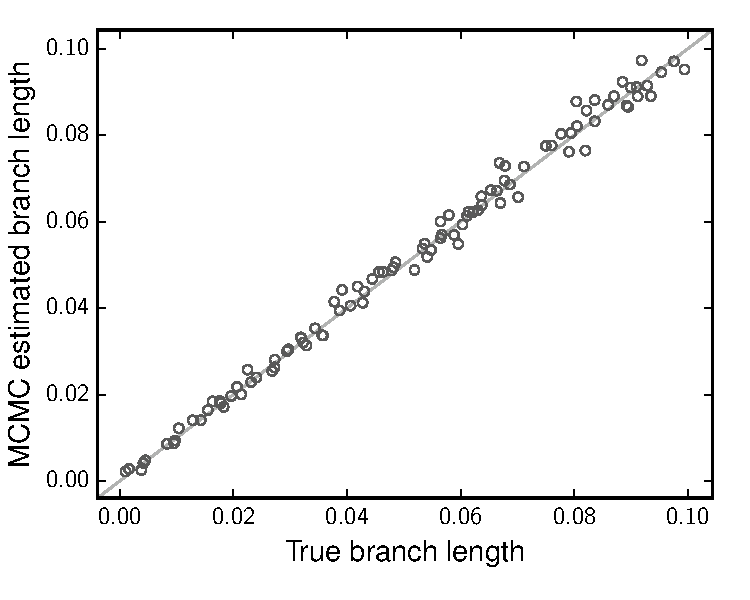
\includegraphics[width=\textwidth]{images/mcmc-branch-length-plot.pdf}
        \caption{B}
    \end{subfigure}
    \captionsetup{name=Figure S, labelformat=noSpace, listformat=sFigList}
    \caption{A comparison of the true branch length separating each pair of
        simulated sequences to the branch length estimated by (A) ABC-GLM and
        (B) full-likelihood MCMC.}
    \label{fig:branchLengthEstimates}
\end{figure}


\end{document}
